\subsection{Dimensão real e financeira do mercado imobiliário}

%%%%%%%%%%%%%%%%%%%%%%%%%%%%%%%%% APRESENTAÇÃO DO PROBLEMA %%%%%%%%%%%%%%%%%%%%%%%%%%
% Apresentação da velha narrativa %
Há um relativo consenso na literatura \textit{mainstream} de que a concessão de crédito às famílias com pior avaliação de risco está na origem da Grande Recessão\footnote{
Um exemplo deste consenso é o livro de \textcite{mian_consequences_2009}.
}. 
% Apresentação do geral: Jordà %
%Partindo de uma base de dados inédita, \textcite{jorda_great_2016} reportam que o crédito concedido às famílias cresceu a uma taxa maior do que para os demais setores não-financeiros de modo que  a intermediação financeira tem alterado o \textit{locus} do risco para os empréstimos imobiliários e hipotecas e que esta dinâmica contribui para a ocorrência de crises financeiras \cite{schularick_credit_2012}.
% Apresentação do específico: nova narrativa %
No entanto, evidências recentes sugerem uma ``nova narrativa'' \cite{albanesi_credit_2017}: os agentes melhor avaliados pelos bancos foram aqueles que adquiriram imóveis para fins especulativos/diversificação de portfólio e apresentaram maiores taxas de \textit{default}; enquanto a concessão de crédito e a taxa de \textit{default} entre aqueles com pior avaliação de risco se mantiveram constantes ao longo da bolha imobiliária.
% TODO Marcar daqui até o fim. Fala que tem um backup da versão anterior. 
Este resultado decorre, em um primeiro momento, da valorização dos imóveis como colateral seguido do esgotamento da bolha imobiliária (pós-2005).
A subsequente desvalorização destes ativos não foi acompanhada pela redução dos compromissos financeiros das famílias (dívida). 
% Backup: Este resultado está associado tanto à valorização dos imóveis como colateral quanto ao descolamento entre os ativos e passivos  das famílias ao longo da crise. Este descolamento decorre tanto do esgotamento da bolha dos imóveis (pós-2005) que fez com que os tais ativos desvalorizassem quanto da insensibilidade dos compromissos financeiros das famílias (dívida) a queda do preço de seus ativos.
Em outras palavras, os imóveis (ativo) têm valor de mercado enquanto a dívida (passivo) tem um valor contratual de modo que o patrimônio líquido das famílias cai  enquanto sua fragilidade financeira aumenta com o instaurar da crise \cites{albanesi_credit_2017}{jorda_rate_2019}.
%O movimento subsequente é caracterizado pelo que \textcite{koo_holy_2009} denominou de ``recessão de balanço patrimonial'' (no original, \textit{balance sheet recession})  em que parte considerável da poupança das famílias é destinada ao pagamento de amortização da dívida para se desalavancar e isso tem implicações negativas para a retomada\footnote{Originalmente, este conceito foi desenvolvido no contexto do estouro da bolha imobiliária no Japão nos anos 1990 e recentemente tem sido utilizado para explicar o pós-Grande Recessão.}.


%%%%%%%%%%%%%%%%%%%%%%%%%%%%%%%%%%%%%%%%% RELEVANCIA DO SFC %%%%%%%%%%%%%%%%%%%%%%%
Dentre os poucos economistas que anteciparam a Grande Recessão, \textcite{godley_seven_1999} se destaca pela sua contribuição metodológica: a abordagem consistente entre fluxos e estoques (adiante, SFC)\footnote{Cabe ressaltar que apesar da metodologia SFC ter recebido uma maior atenção no pós Grande Recessão, é uma proposta de análise cujas origens datam desde os anos 70. Sobre as origens desta metodologia, suas hipóteses explícitas e implícitas, ver \textcite{teixeira_crescimento_2015}.}.
Nos últimos anos, houve um crescente consenso na literatura heterodoxa de que esta metodologia é uma das melhores formas de modelar a conexão do lado real ao financeiro da economia \cite{nikiforos_stock-flow_2017}.
% Lacuna 1: poucos olham investimento residencial %
Apesar da crescente aceitação desta metodologia pela literatura, os imóveis estão entre os ativos menos analisados  \cite{caverzasi_stock-flow_2013}.
%% Petrini e Teixeira %
Uma exceção é o modelo de \textcites{petrini_demanda_2019}{petrini_long_2020} em que são incluídos crédito às famílias e firmas; investimento residencial e bolha de ativos.
Diferente de \textcite{zezza_u.s._2008} e \textcite{nikolaidi_securitisation_2015}, os autores partem do supermultiplicador sraffiano de modo que é o investimento residencial que lidera o ciclo econômico\footnote{
    Desenvolvido originalmente por \textcite{serrano_sraffian_1995}, o supermultiplicador sraffiano tem sido utilizado por um conjunto de autores mais amplo como é o caso de \textcites{allain_tackling_2015}{lavoie_convergence_2016}{serrano_sraffian_2017}{dutt_observations_2018} e, mais recentemente, sido incluído na estrutura contábil SFC por \textcites{brochier_supermultiplier_2018}{mandarino_workers_2020}.
}.
Sendo assim,  tal modelo enfatiza as implicações das bolhas de ativos (neste caso, imóveis) sobre o crescimento econômico e acumulação de capital.
Apesar de analisar as implicações macroeconômicas do investimento residencial, o modelo de \textcite{petrini_demanda_2019} carece de uma melhor representação da relação entre o mercado imobiliário e de crédito, bem como composição patrimonial dos bancos e esta é uma das lacunas a ser preenchida por esta pesquisa.


%Partindo de uma base de dados inédita, \textcite{jorda_great_2016} reportam que o crédito concedido às famílias cresceu a uma taxa maior do que para os demais setores não-financeiros de modo que  a intermediação financeira tem alterado o \textit{locus} do risco para os empréstimos imobiliários e hipotecas e que esta dinâmica contribui para a ocorrência de crises financeiras \cite{schularick_credit_2012}.
%Desse modo, 
Para dar conta das implicações reais e financeiras da macroeconomia imobiliária, se faz necessário compreender as relações entre a composição patrimonial dos bancos e a fragilidade financeira das famílias.
Uma literatura que dá atenção a alguns desses temas é a que parte das contribuições de Hyman Minsky.
Na literatura, somente o trabalho de \textcite{ryoo_household_2016} relaciona o endividamento e a fragilidade financeira das famílias às bolhas de ativos \cite{nikolaidi_minsky_2017}. 
%Ao avaliar esta famílias de modelos que seguem a metodologia SFC, \textcite{nikolaidi_minsky_2017} identificam somente o trabalho de \textcite{ryoo_household_2016} analisa o endividamento e a fragilidade financeiras das famílias conjuntamente. 
Neste modelo, são os trabalhadores --- e não os rentistas --- que investem em imóveis e o fazem a partir da taxa de retorno esperada ao se especular com casas\footnote{Cabe destacar que o trabalho de \textcite{ryoo_household_2016} se baseia em normas estoque-fluxo exogenamente determinadas de modo que ciclos financeiros no modelo também se tornam exógenos.}.
Apesar de avançar em direção a um maior esclarecimento na relação entre bolha de ativos e instabilidade financeira das famílias, as hipóteses do modelo de \textcite{ryoo_household_2016} podem ser questionadas uma vez que \textcite{albanesi_credit_2017} encontraram evidências empíricas de que foram os rentistas ---  e não os trabalhadores --- que especularam com imóveis.
%TODO: Marcar
%%%%%%%%%%%%%%%%%%%%%%%%%%%%%%%%%%%%%%%%% LACUNA SFC %%%%%%%%%%%%%%%%%%%%%%%%%%%%%%%


A partir da revisão de literatura dos modelos SFC, nota-se o pouco detalhamento das relações financeiras entre famílias e bancos \cite{lavoie_was_2020}. %TODO Marcar. Obtei tirar as firmas dessa frase tb. Achei que tirava mto o foco.
Outra lacuna identificada na literatura que parte desta metodologia é o tratamento teórico do setor financeiro em que atua como intermediador bancário \cite{le_heron_post-keynesian_2008}\footnote{\textcite{nikolaidi_minsky_2017} também destacam que a maioria dos modelos minskyanos que partem da metodologia SFC enfatiza o endividamento das firmas e o fazem sem incluir racionamento de crédito.}.
Portanto, os modelos SFC têm dado pouca atenção à relação entre fragilidade financeira das famílias, investimento residencial, racionamento de crédito e bolha de ativos. 
%%%%%%%%%%%%%%%%%%%%%%%%%%%%%%%%%%%%%%%%% LACUNA SFC E COMPLEMENTARIEDADE ABM %%%%%%%%%%%%%%%%%%%%%%%%%%%


Seguindo \textcite{bellofiore_minskys_2001}, destaca-se que a melhor forma de analisar fenômenos como a instabilidade financeira minskyana é por meio de modelos que possuem agentes com comportamentos heterogêneos como é o caso da modelagem baseada em agentes (adiante, ABM).
%%%%%%%%%%%%%%%%%%%%%%%%%%%%%%%%%%%%%%%% LACUNA ABM NÂO SFC%%%%%%%%%%%%%%%%%%%%%%%%%%%%%%%%
%%%%%%%%%%%%%%%%%%%%%%%%%%%%% AB-SFC COM CICLO ENDÓGENO %%%%%%%%%%%%%%%%%%%%%%%%
Uma forma de incluir racionamento de crédito nesta metodologia é a de \textcite{dawid_bubbles_2015} em que os autores analisam as relações entre regulação bancária e ciclo econômico.
No entanto, tal como é usual nesta literatura, racionamento de crédito é exclusivo à relação entre firmas e bancos, enquanto as famílias apenas acumulam riqueza sob a forma de depósitos bancários.
Outros autores que utilizam modelos do tipo ABM têm avaliado as relações entre instabilidade financeira, endividamento das famílias e distribuição de renda.
\textcite{cardaci_inequality_2018} parte da hipótese de consumo cascata para investigar as associações entre a concentração da renda e inflação de imóveis\footnote{
    Em linhas gerais, a hipótese de consumo cascata desenvolvida por \textcite{duesenberry_income_1949} descreve que o aumento do consumo dos percentis mais elevados de renda induzem o aumento do consumo dos percentis inferiores e este efeito é maior quanto maiores forem as disparidades de renda. %\textcite{veblen_theory_1899}
}.
Apesar de relevante, tal contribuição não avança em direção a uma especificação dos determinantes da taxa de crescimento do investimento residencial.
Além disso, tanto \textcite{dawid_bubbles_2015} quanto \textcite{cardaci_inequality_2018} não mapeiam explicitamente as relações entre fluxos e estoques como propõe a metodologia SFC.


%%%%%%%%%%%%%%%%%%%%%%%%%%%%%%%%%%%%%%% RELEVÂNCIA AB-SFC %%%%%%%%%%%%%%%%%%%%%%%%%%
Uma alternativa é o modelo de \textcite{caiani_agent_2016} em que os autores propõem um ABM na estrutura contábil SFC (adiante, AB-SFC) de modo a desfrutar das vantagens de ambas metodologias: emergência de fenômenos macroeconômicos em que estão explicitados todos os \textit{feedbacks} intersetoriais entre fluxos e estoques.
Por mais que o modelo de \textcite{caiani_agent_2016} seja bastante desagregado e detalhado, não inclui tanto bolha de ativos e investimento residencial quanto relações de crédito entre famílias e bancos.
%%%%%%%%%%%%%%%%%%%%%%%%%%%%% AB-SFC PARCIAL, SEM IMÓVEIS %%%%%%%%%%%%%%%%%%%%%%
Uma forma de explicitar as relações entre fluxos e estoques e incluir heterogeneidade dos agentes sem precisar incorrer em um elevado grau de desagregação é por meio de um modelo AB-SFC parcial em que somente alguns agentes possuem comportamento heterogêneo.
Além de ser mais parcimonioso, tal procedimento permite evidenciar a emergência de interações complexas entre os agentes sem que, para isso, seja necessário abrir mão da compreensibilidade do modelo.
Um exemplo desta estratégia é o modelo de \textcite{botta_when_2019} em que os autores investigam as implicações da complexidade financeira na presença de famílias heterogêneas com restrição de crédito.
\textcite{carvalho_income_2014} também elaboram um modelo AB-SFC parcial em que o setor das famílias é heterogêneo para investigar a estabilidade da dinâmica de endividamento deste setor e as relações entre distribuição funcional e pessoal da renda.
Apesar de ambos modelos lançarem luz sobre as relações entre famílias heterogêneas e bancos na presença de racionamento de crédito, não analisam a fragilidade financeira das famílias e também não 
incluem investimento residencial nem bolha de ativos. 


%%%%%%%%%%%%%%%%%%%%%%%%%%%%%%%%%%%%%%% LACUNA AB-SFC %%%%%%%%%%%%%%%%%%%
Dessa forma, enquanto os modelos SFC são mais adequados para investigar as relações entre setor real e financeiro, nota-se a pouca ênfase à possibilidade de racionamento de crédito e de um sistema bancário ativo. %TODO Marcar.
Além disso, por se tratar de uma metodologia ao nível agregado, não é capaz de tratar de questões relativas à fragilidade financeira minskyana de forma adequada, conforme destacam \textcite{bellofiore_minskys_2001}.
Já os modelos ABM, mais adequados para investigar instabilidade financeira, dão pouca ênfase às famílias e esta lacuna se estende aos modelos AB-SFC.
Pontua-se ainda a pouca atenção dada ao investimento residencial nas abordagens mencionadas.
Percebe-se, portanto, que a literatura não tem investigado conjuntamente os temas aqui elencados sob o título de macroeconomia imobiliária.

%%%%%%%%%%%%%%%%%%%%%%%%%%%%% PROPOSTA: AB-SFC PARCIAL, COM IMÓVEIS %%%%%%%%%%%%%%%%%%%%%%
Dito isso, a presente pesquisa propõe um modelo AB-SFC com investimento residencial e bolha de ativos em que as famílias são heterogêneas.
Portanto, o modelo a ser elaborado se distingue de \textcite{petrini_demanda_2019} ao desagregar as famílias;
de \textcite{dawid_bubbles_2015} e \textcite{caiani_agent_2016} ao enfatizar as relações entre famílias e bancos na presença de racionamento de crédito;
de \textcite{botta_when_2019} e \textcite{carvalho_income_2014} ao incluir investimento residencial e; de \textcite{zezza_u.s._2008} e \textcite{nikolaidi_securitisation_2015} uma vez que tal gasto lidera o crescimento econômico.
Sendo assim, trata-se de um modelo AB-SFC parcial com famílias heterogêneas, dois ativos reais (capital das firmas e imóveis), racionamento de crédito e inflação de imóveis.


\begin{comment}
No que diz respeito aos modelos teóricos analisados, nota-se a pouca atenção às famílias e uma maior ênfase à relação entre firmas e bancos \cite{lavoie_was_2020}.
Nos modelos \textit{Stock-Flow Consistent}, por exemplo, o setor financeiro atua como um mero intermediador bancário \cite{le_heron_post-keynesian_2008} e dentre os modelos \textit{Agent Based} (adiante, ABM) com setor bancário ativo, a concessão de crédito se restringe quase sempre às firmas  \cite{delli_gatti_financial_2003}.



Nos Estados Unidos (EUA), o início dos anos 2000 é marcado por momentos bastante distintos. Logo em 2001, a economia é atingida pela crise das bolhas-ponto-com com a possibilidade de uma recessão. No entanto, a recuperação foi rápida e seguida de um ciclo de crescimento que se estendeu de 2002 a 2007 \cite{cagnin_o_2007}.  Por mais que a economia americana seguiu crescendo até 2007, o investimento residencial iniciou a reversão já em 2005. Ao longo deste período, os demais componentes da demanda agregada contribuíram para o adiamento da crise, mas não foram suficientes para impedir o colapso do investimento residencial ocorrido em 2008. 
Apesar desta dinâmica sugerir uma atipicidade, segue um padrão bem definido para o caso norte-americano, qual seja, o ciclo econômico é liderado pelo investimento residencial \cites{green_follow_1997}{leamer_housing_2007}{fiebiger_trend_2017}\footnote{
Ao avaliar o caso norte-americano, \textcite{green_follow_1997} conclui que o investimento residencial antecipa o ciclo econômico, mas que isso não implica no estabelecimento de uma relação causal. 
}.


Como será discutido adiante, a abordagem SFC é compatível inúmeras teorias e propostas apesar do arcabouço contábil rígido. 
A mesma variabilidade de temas possíveis de serem abordados pela metodologia SFC se estende para a pluralidade dos ativos passíveis de serem incorporados e ao grau de complexidade financeira de cada modelo. 
Ao mapearem os ativos mais frequentes na literatura, \textcite[p.~4]{caverzasi_stock-flow_2013} mostram os imóveis são os ativos menos modelados, sendo o ativo menos estudado. 


Vale ressaltar que a partir do estabelecimento do SSM, algumas questões são colocadas: quais são esses gastos autônomos e quais seus determinantes? Qual o padrão de financiamento e suas consequências? \textcite{pariboni_household_2016} e \textcite{fagundes_dinamica_2017}, por exemplo, avançaram em detalhar o consumo financiado por crédito.  \textcite{brochier_supermultiplier_2018}, por sua vez, incorporam o SSM em uma estrutura contábil mais completa, o arcabouço de consistência entre fluxos e estoques (SFC, na sigla em inglês), para compreender a dinâmica do consumo a partir da riqueza. 

Nesta família de modelos: 
(i) o grau de utilização converge ao grau normal (planejado pelas firmas) no longo prazo; 
(ii) a distribuição renda não influencia o crescimento de longo prazo; 
(iii) o investimento das \textbf{firmas} segue o princípio de ajuste do estoque de capital e;
(iv) o ajuste do estoque de capital é feito de forma tênue e gradual. 


\begin{figure}[htb]
	\centering
	\caption{Mapa de calor dos ativos modelados com SFC}
	\label{Heatmap}
	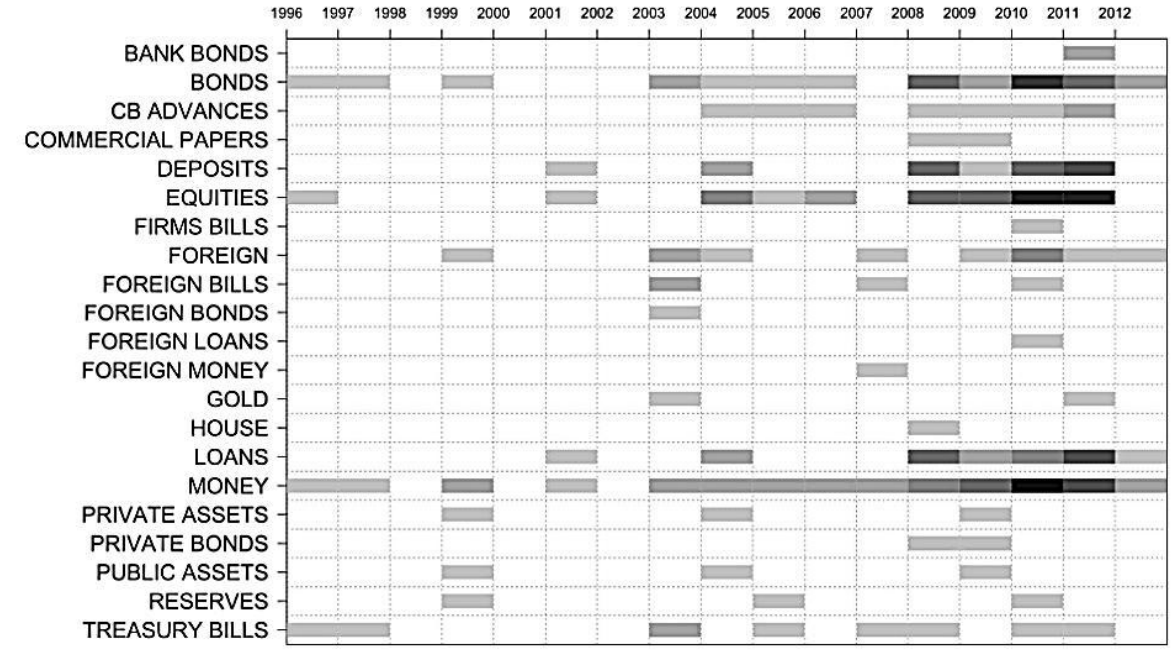
\includegraphics[width = 0.9\textwidth]{./figs/Caverzassi_Heatmap.png}
	\caption*{\textbf{Fonte:} \textcite[p.~4]{caverzasi_stock-flow_2013}}
\end{figure}


Compreendidas tais relações, será desenvolvido um modelo SSM-SFC para dar conta das relações entre lado real e financeiro da economia.
Portanto, esta pesquisa segue o caminho aberto por \textcite{brochier_supermultiplier_2018} ao adicionar um tratamento adequado das relações financeiras no SSM por meio da metodologia SFC estendendo as contribuições de: 
(i) \textcite{jorda_great_2016} ao investigar o processo de ``hipotecarização'' sob um prisma pós-keynesiano a partir de uma análise qualitativa comparativa (QCA); 
%(ii) \textcite{serrano_sraffian_1995} ao incluir o investimento residencial na agenda de pesquisa do supermultiplicador sraffiano; 
(ii) \textcite{teixeira_crescimento_2015} ao avaliar a aplicabilidade da taxa própria de juros dos imóveis para além dos Estados Unidos e;
(iii) \textcite{da_silveira_investimento_2019} ao conectar as relações entre o mercado imobiliário e de crédito diante das especificidades institucionais destacas anteriormente por meio de um modelo SFC de simulação. 




\begin{quote}
	\textit{On the one hand, the German housing
		market was one of the few markets in Western Europe that was not severely affected by the
		global housing boom of the early 2000s. On the other hand, recent developments suggest
		that the role of finance in the German housing system is \textbf{changing}, but not in the same way as
		in other countries}. \cite[p.~969, grifos adicionados]{wijburg_alternative_2017}
\end{quote}

\footnote{Apenas para ilustrar a pluralidade de temas que tal metodologia já abordou, temos --- mesmo que em sua forma mais originária encontrada em \textcite{godley_macroeconomics_1983} --- as formas de financiamento das firmas \cites{asimakopulos_kalecki_1983}{skott_finance_1988}{messori_financing_1991}; endogeneidade da moeda e importância do sistema bancário \cites{messori_financing_1991}{dow_horizontalism:_1996}{arestis_theoretical_1996}{godley_money_1999}; endividamento, distribuição de renda e, apenas para restringir os temas, financeirização \cites{palley_inside_1996}{wolfson_irving_1996}{palley_money_1997}{palley_financial_2002}{dos_santos_revisiting_2009}{palley_inside_2010}{hein_finance-dominated_2012}.}

Sendo assim, o investimento residencial no trabalho de \textcite{nikolaidi_securitisation_2015} possui tanto uma parcela autônoma em relação à renda quanto outra induzida pela renda disponível das famílias.
No entanto, ao partir do procedimento de \textcite{godley_money_1999} para determinação do portfólio de ativos dos agentes, trata os imóveis como um ativo financeiro qualquer sem considerar suas particularidade, qual seja, durabilidade e baixo risco. %TODO: Rever particularidade dos imóveis.


Um  exemplo é o trabalho de  em que são investigados os efeitos da diminuição --- apesar da distribuição da renda a favor dos lucros --- da propensão média a poupar da economia norte-americana por meio da introdução do mercado imobiliário na metodologia SFC\footnote{
	Tal resultado, argumenta, decorre dos ganhos de capital nos mercados imobiliário e acionário entre o topo da distribuição, contribuindo para a diminuição da taxa de poupança.
}. 
Por mais que este trabalho seja uma via para a inclusão do investimento residencial nos modelos macroeconômicos, tal gasto não é o principal determinante da dinâmica  uma vez que parte de uma especificação kaleckiana do investimento das firmas.
Sendo assim, 

Alguns trabalhos seguiram a contribuição de \textcite{zezza_u.s._2008}.
Um deles é o de  com dois tipos de agentes demandando imóveis: parcela dos trabalhadores e investidores institucionais.
Para os primeiros, a demanda por casas é determinada positivamente pela poupança deste setor acrescido de empréstimos hipotecários e negativamente pelo preço dos imóveis de modo que não pode ser considerado estritamente autônomo.
Já os demais agentes, demandam imóveis tal como outros ativos financeiros, ou seja, depende positivamente de sua taxa de retorno.
Em conjunto, tais equações comportamentais determinam que a taxa de crescimento do investimento residencial depende tanto da razão entre a demanda por imóveis em relação ao total quanto de sua inflação que, por sua vez, é determinada pelo estoque de imóveis não vendidos.


%%%%%% ANÁLISE INSTITUCIONAL COMPARATIVA A PARTIR DA NEI -> CHANG: CONFIGURAÇÕES DIFERENTES LEVAM ÀS MESMAS FUNÇÕES. %%%%
A literatura sobre análise institucional comparada se deve, em grande medida, aos desenvolvimentos da Nova Economia Institucional (MENARD e SHIRLEY).
Tal abordagem, no entanto, não faz uma distinção entre formas e funções das instituições além de partir do paradigma ``one-fits-all'' (CHANG 2007, Ch2).
CHANG 2011, por outro lado, argumenta que  diferentes arranjos institucionais podem desempenhar (conjuntamente) as mesmas funções. 
Dito isso, a presente pesquisa parte desta hipótese de ausência de uniformidade causal do arranjo institucional e, assim, enfatizará as particularidades de cada país.



\end{comment}